\documentclass{betterposter}

\usepackage[default]{lato}
\usepackage{inconsolata}

\usepackage{fontawesome}
\usepackage{graphicx}

\definecolor{mygrey}{RGB}{63, 63, 63}

% Title font
\renewcommand{\fontsizetitle}{\fontsize{64}{80} \selectfont}

% Main column font
\renewcommand{\fontsizemain}{\fontsize{125}{200} \selectfont}

%% Setting the width of columns
% Left column
\setlength{\leftbarwidth}{0.25\paperwidth}
% Right column
\setlength{\rightbarwidth}{0.25\paperwidth}

\begin{document}
\color{mygrey}

\betterposter{%

%%% MAIN COLUMN %%%
\maincolumn{%
    \textbf{Benchmark datasets} are \textbf{not the only option} when
    \textbf{understanding} an algorithm's \textbf{performance}
}{%
    \compactqrcode{img/paper_qr.eps}{%
        \textbf{Take a picture} to\\
        download the full paper
    }%
    \hfill%
    
\includegraphics[width=.3\linewidth]{img/cu_logo}

    \vfill%
    \textbf{%
        \faGithub~\faTwitter\ \ daffidwilde
        \hfill%
        \faBook\ \ \texttt{edo.readthedocs.io}
        \hfill%
        \faNewspaperO\ \ \texttt{arxiv.org/abs/1907.13508}
    }
}

}{%

%%% LEFT COLUMN %%%
\title{Evolutionary dataset\\optimisation: \textit{learning\\algorithm quality
through evolution}}
\author{\textbf{Henry Wilde}, Vincent Knight,\\ Jonathan Gillard}

\section{Motivating paradigm}

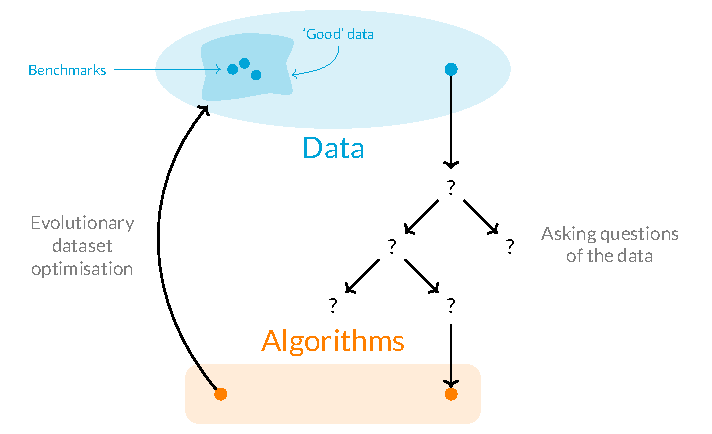
\includegraphics[width=\linewidth]{tex/paradigm.pdf}


\section{Using an evolutionary\\algorithm}

\begin{minipage}{.05\linewidth}
    \
\end{minipage}
\begin{minipage}{.9\linewidth}
\begin{itemize}
    \renewcommand\labelitemi{\faThumbsOUp~}
    \item Effective in complex domains
    \item Adjustable design
    \item Transparent and rich solutions
\end{itemize}

\vspace{1ex}\begin{itemize}
    \renewcommand\labelitemi{\faThumbsODown~}
    \item Potential suboptimal termination
    \item Finds the `easy' way out
    \item Requires careful consideration of fitness
\end{itemize}
\end{minipage}


\section{A case study in clustering}

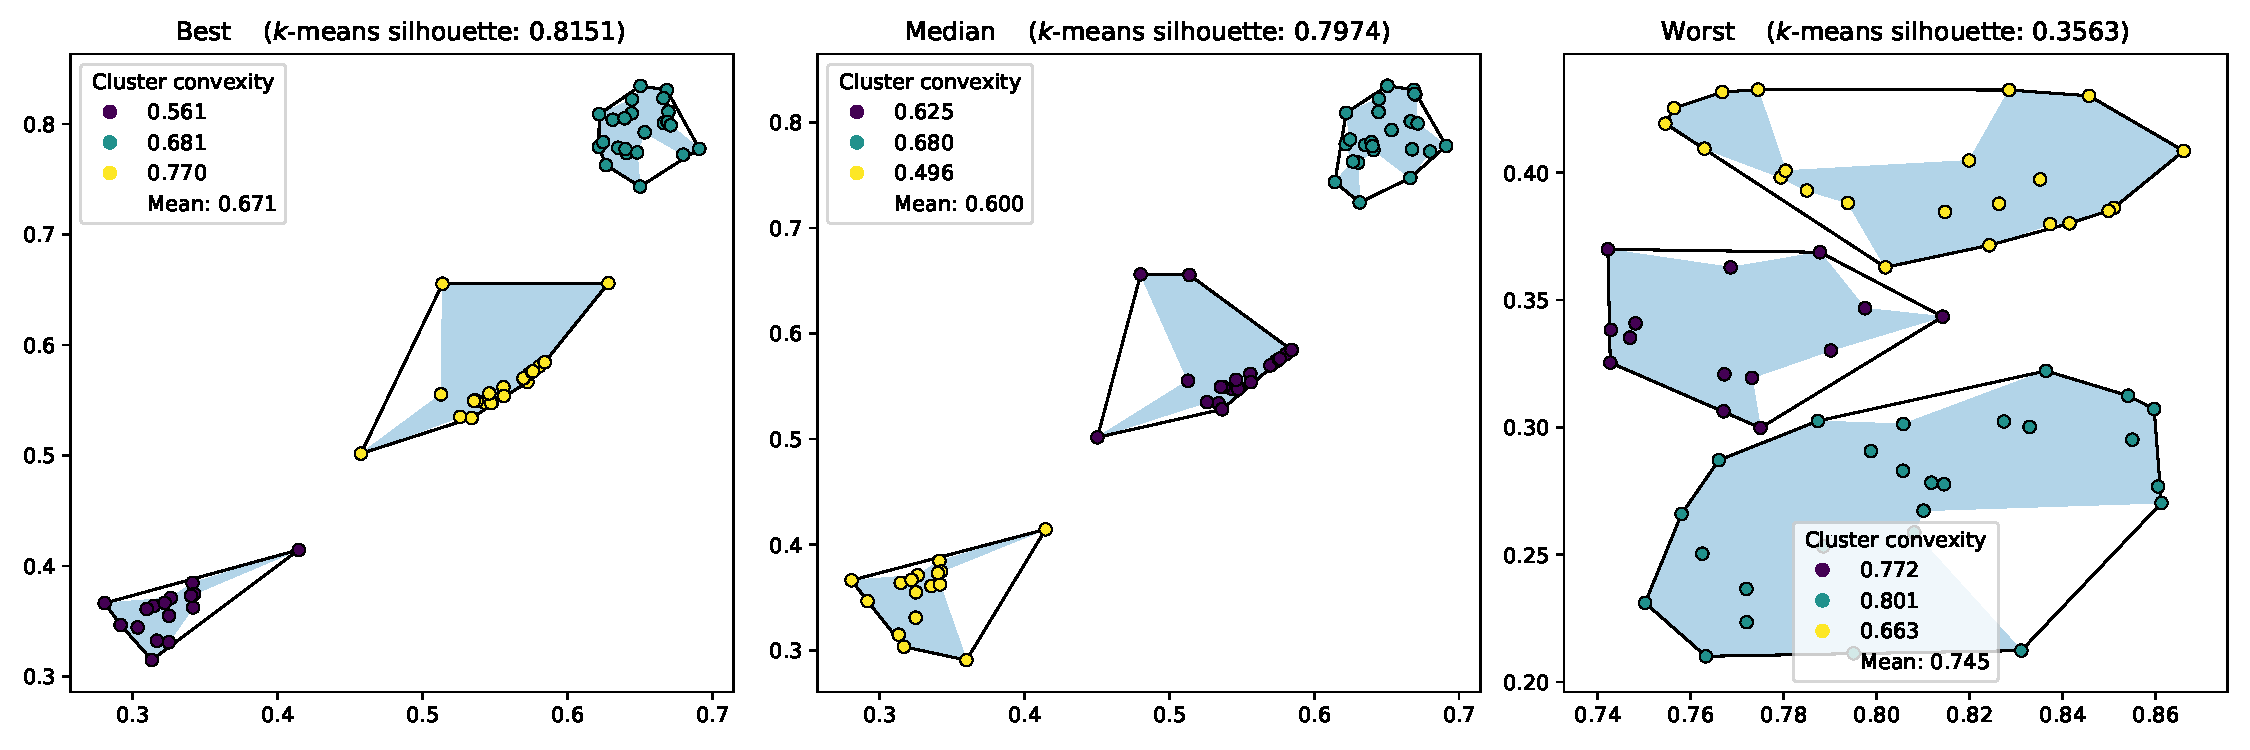
\includegraphics[width=\linewidth]{img/kmeans.pdf}\vspace{1ex}

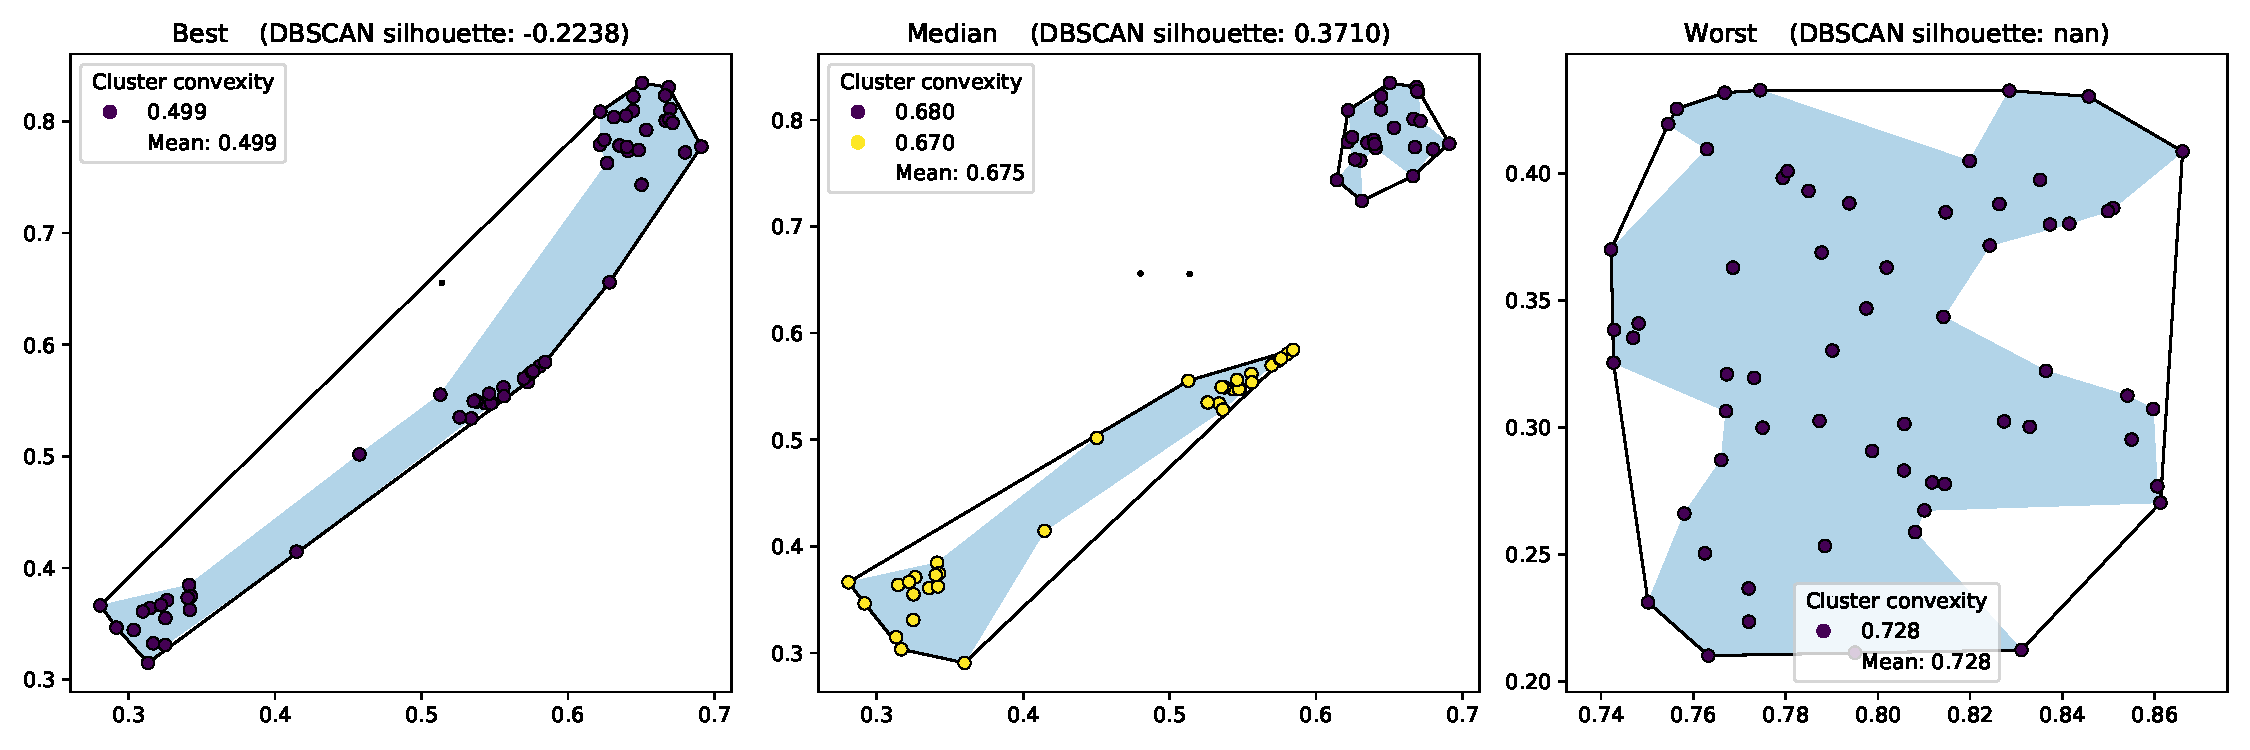
\includegraphics[width=\linewidth]{img/dbscan.pdf}

}{%

%%% RIGHT COLUMN %%%

\vspace{-2em}\section{Inner mechanisms}

\centering%
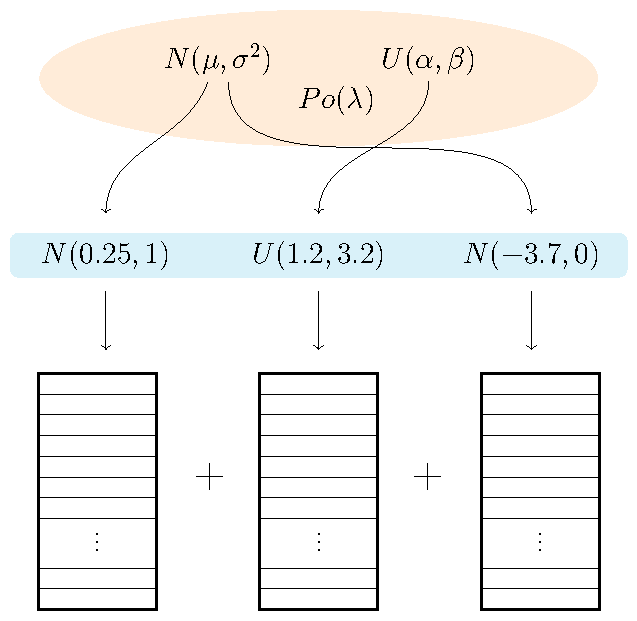
\includegraphics[width=.6\linewidth]{tex/individual.pdf}
\vfill\vspace{.5ex}\hrule height 3pt\vspace{.5ex}\vfill

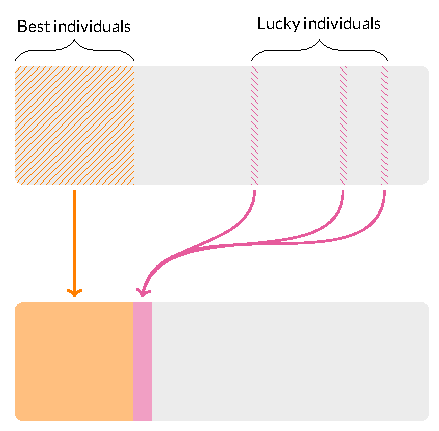
\includegraphics[width=.5\linewidth]{tex/selection.pdf}
\vfill\vspace{.5ex}\hrule height 3pt\vspace{.5ex}\vfill

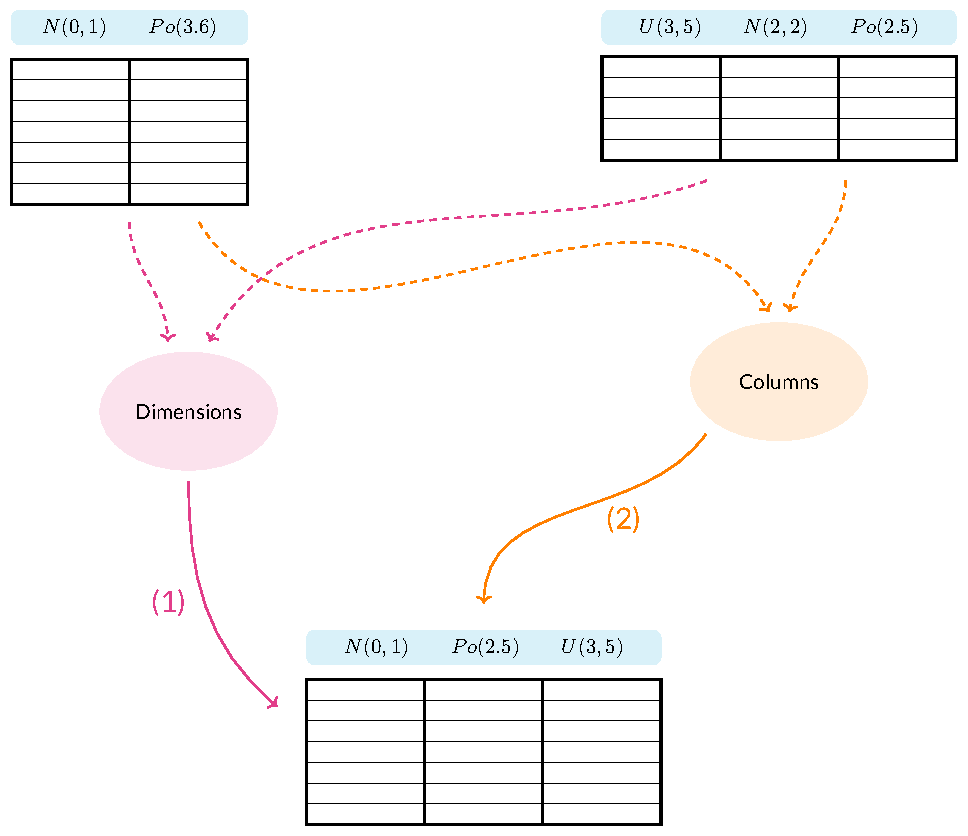
\includegraphics[width=.8\linewidth]{tex/crossover.pdf}
\vfill\vspace{.5ex}\hrule height 3pt\vspace{.5ex}\vfill

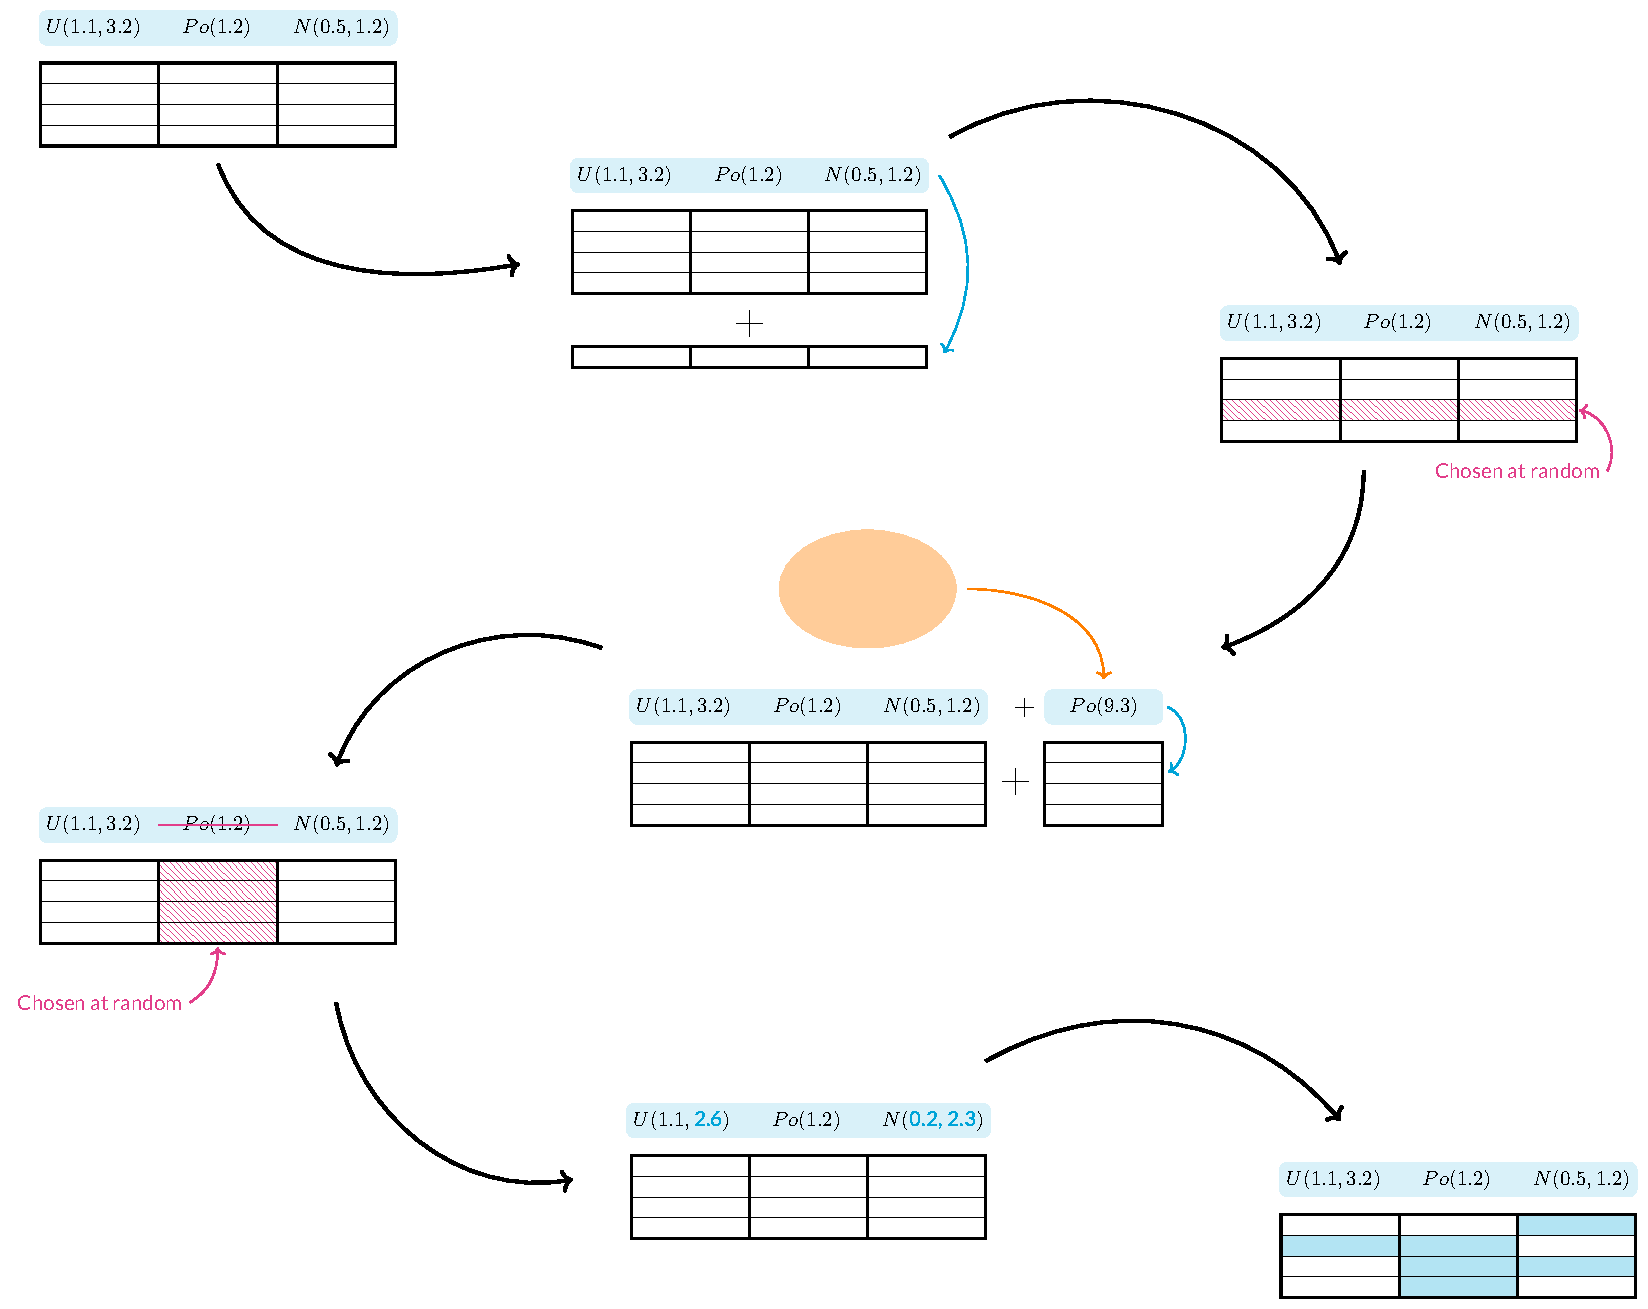
\includegraphics[width=\linewidth]{tex/mutation.pdf}

}

\end{document}
